\documentclass[12pt, a4paper, onecolumn]{article}
\usepackage{fontspec}
\usepackage{titlesec}
\usepackage{tocloft}
\usepackage[english]{babel}
\usepackage{blindtext}
\usepackage{subfig}
\usepackage{pgf}
\setmainfont{Georgia}

\newcommand\sectionfont{\normalfont\fontspec{Arial}\fontsize{14pt}{0}\bfseries}
\newcommand\subsectionfont{\normalfont\fontspec{Arial}\fontsize{13pt}{0}\bfseries}
\newcommand\subsubsectionfont{\normalfont\fontspec{Arial}\fontsize{12pt}{0}\bfseries}
\newcommand\tocsectionfont{\normalfont\fontspec{Arial}\fontsize{12pt}{0}\bfseries}
\newcommand\tocsubsectionfont{\normalfont\fontspec{Arial}\fontsize{11pt}{0}\bfseries}
\newcommand\tocsubsubsectionfont{\normalfont\fontspec{Arial}\fontsize{11pt}{0}}
\newcommand\toctitlefont{\normalfont\fontspec{Arial}\fontsize{16pt}{0}\bfseries}


\titleformat{\section}{\sectionfont}{\thesection}{20pt}{}
\titleformat{\subsection}{\subsectionfont}{\thesubsection}{20pt}{}
\titleformat{\subsubsection}{\subsubsectionfont}{\thesubsubsection}{20pt}{}

\renewcommand{\cftsecfont}{\tocsectionfont}
\renewcommand{\cftsubsecfont}{\tocsubsectionfont}
\renewcommand{\cftsubsubsecfont}{\tocsubsubsectionfont}
\renewcommand{\cftsecpagefont}{\tocsectionfont}
\renewcommand{\cftsubsecpagefont}{\tocsubsectionfont}
\renewcommand{\cftsubsubsecpagefont}{\tocsubsubsectionfont}
\renewcommand{\cfttoctitlefont}{\toctitlefont}


\addto\captionsenglish{
	\renewcommand{\contentsname}{Table of Contents}
}





\begin{document}
	
	\tableofcontents
	\newpage

\subsection{Problem}

Falling accidents are common, as described in the background, and it is important that a person who suffers an accident, is aided as quickly as possible to minimize the consequences of the accident. Since a person who suffers a fall may end up in a situation where the person is unable to call for help, for example, because the person is injured or unconscious, an application that could send an automatic alarm could be of great use. An automatic alarm would help minimize the time between the accident and help arriving, since without the alarm, it could take a long time before the person is found by passers-by. For this reason, we want to investigate the possibility of creating a mobile application that can detect falling accidents and report to registered contacts. A mobile application has the advantage that most people already have a smart phone, so if a mobile application could accomplish the task successfully, the cost would be minimized since there will be no need for additional hardware.

This leads us to wonder if it is possible to create such an application, it may be difficult to achieve accuracy in fall detection using only the sensors in the mobile phones that exists on the market today. And if falls were successfully detected, would it be possible to filter out other activities in daily life that resembles falls such as running, jumping or sitting down fast and remain only with the actual falling accidents?

Another question that arises is the fact that this kind of application may have a significant impact on battery life, since it would be necessary to continuously read the sensor values. If the application would drain the battery on the mobile phone, it would make the application far less valuable, since it is unlikely that it would be used.

\subsection{Problem Statement}

This study will aim to answer the questions:

\begin{itemize}
	\item Is it possible to create a mobile application that accurately detects falling accidents using the sensors available in smart phones on the market today?
	\item How will such an application affect the battery life of the mobile phone?
\end{itemize}

	
\subsection{Methodologies / Methods}

The first part of the research will be to perform a literature study, where we will gain deeper knowledge in the subject, and find out what earlier attempts have been made to solve this problem. The literature study will give a good starting point for the rest of the study. The next step will be a case study where we develop a mobile application that uses sensors available in smart phones to achieve accurate fall detection. Developing such an application will give us the opportunity to test theories and ideas found in the literature study. Lastly, the applications impact on battery life will be tested by performing experiments using mobile phones running the application.   

\section{Methodologies and Methods}

This chapter describes the research strategy and the methodologies used in the study, and how each methodology will contribute to the research question.

\subsection{Research Strategy}



\subsubsection{Research Methods}

\paragraph{Literature Study}
The literature study that we will perform will focus on finding an answer for the first question in the problem statement, which algorithm should be used to accurately detect a fall. The result of the literature study will show which algorithm for fall detection that would be proposed by earlier studies. This algorithm will serve as a starting point for our own implementation, where we will try to improve the algorithm. The outcome of the literature study is presented in the theoretical background.

\paragraph{Developing a mobile application}
The second part of our research will be a case study where we implement a fall detection system for Android and iOS. This application will use the algorithm found in the literature study, and try to give an answer to the second question in our problem statement. Developing the application will give us an opportunity to test the algorithm on real devices, and a platform where we can experiment in order to improve the algorithm. The result of the development will try to give an answer to the second question in our problem statement, how can technology available in smart phones be used to implement the algorithm found in the literature study.

\paragraph{Evaluating the implemented mobile application}

The third part of our research will be to evaluate the implemented algorithm by performing experiments where the mobile application is used to detect falls. The evaluation will try to give an answer to the third question in our problem statement, how performance issues can be minimized.

\subsubsection{Research Process}

In this thesis project, the work is divided in phases. The first phase, the problem statement serves to formulate the problem that the thesis will try to solve. The second phase is the literature study, where reports from earlier studies are collected and read to give us a deeper understanding of the subject. The third phase is the analysis phase, where the results of the literature study is analysed in order to find an algorithm that will be suitable as a starting point for the application. The next phase is the design phase, where the application development starts. After the design phase comes the implementation phase, where the application is implemented. After the implementation phase, there is the evaluation phase, where the developed application is evaluated. After this phase, in case the application is not good enough or if we have found ideas for improvement of the algorithm the process will go back to design, to implement another version of the application. After the application have been developed, the conclusion phase starts, where the results are summarized and conclusions formulated. 

\begin{figure}[h]
	\centering
	\subfloat{{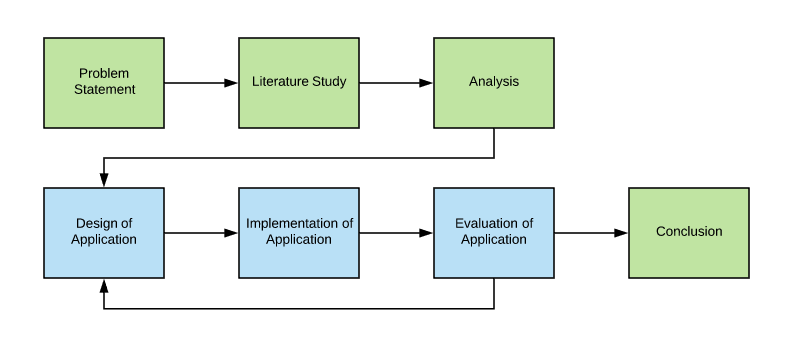
\includegraphics[width=12cm]{../img/Methods.png} }}%
	\caption{The different phases in the thesis project}%
	\label{fig:example}%
\end{figure}

\subsection{Design and Implementation of Application}

\subsubsection{Design of Application}

\subsubsection{Implementation of Application}

To develop the mobile application we will use an iterative development method. By using an iterative method we will make sure that the most important features are developed first, since we will develop the most important features in the first iteration and only after that continue with the less important features. This will help us  minimize the risks in the project. If the project would suffer from lack of time, we would at least have developed the most important features already. The project method that we will be using will be similar to Scrum, although since we are only two developers, the team involved in development will be much smaller than the typical agile team.

We will divide the work in such a way that one of us will develop the Android implementation, and one of us will develop the iOS implementation. By dividing the work in this fashion we can implement similar features in both applications without the risk of writing conflicting code. Another reason for dividing the work is that it will help us to have equal focus on both the Android and iOS implementation.

\subsubsection{Development Environment}

\subsection{Evaluation Methods}

\subsubsection{Evaluating battery life}

To evaluate how the application affects the battery life of the mobile phone, we will use the native functionality in the operating system available on Android and iOS respectively to measure the specific applications power consumption.
In combination with this, we will also perform tests where we run the application for a certain amount of time and note how much battery life is left and compare this value with the percentage left after not running the application for the same amount of time.

\subsubsection{Evaluating the fall detection system functionality}

Another step in the evaluation of the application will be to perform crash tests where we measure how well the application detects a fall, by dropping a mobile phone running the application several times from a height that we define as a fall and count the number of reported falls. The same test can then be performed with an existing application to compare how well the implemented algorithm compares to existing technology.

Another measurement will be to drop the mobile phone running the application from a height that we do not define as a fall, and count how many falls are falsely detected. This number will also be compared the result of running the same test with an existing application.

Yet another test will be to perform daily activities that can trigger a fall detection system, even though it is not a fall. Theses activities can be running, or walking with the phone in the pocket. A good fall detection software will not report many of these false positives. This will also be compared against an existing application.


	   
	\newpage
	
	
	
	\section{The work}
	\newpage
	
	\section{Result}
	\newpage
	
	\section{Conclusions}
	\newpage
	
	
\end{document}